\documentclass{article}
\usepackage[margin=1in]{geometry}
\usepackage{../common}
\usepackage{../pagesetup}

\begin{document}
%\lecture{**LECTURE-NUMBER**}{**DATE**}{**LECTURER**}{**SCRIBE**}
\lecture{3}{October 8}{Nati Srebro}{Shuyan Huang}{VC Theory, No Free Lunch and the Fundamental Theorem of Statistical Learning}

In this lecture, we will introduce VC dimension as a formal way to characterize the number of "parameters" of a hypothesis class. And instead of cardinality, we will give a convergence bound of ERM based on VC dimension. We will also show some examples of calculating VC dimension and introduce half space representation theorem. Finally, we will present statistical no free lunch theorem and give a proof of a stronger statement.

\subsection{Cardinality and Sample Complexity}
We have given a upper bound of sample complexity based on cardinality:
\begin{displaymath}
  m_\mcH(\epsilon, \delta)\leq m_{ERM,\mcH}(\epsilon, \delta)\leq O(\frac{\log{|\mcH|}+\log{1/\delta}}{\epsilon^2})
\end{displaymath}
This shows that all finite hypothesis classes are PAC learnable. However, it remains to be seen whether it is also a necessary condition. If not, there can be infinite classes that are learnable. Also, is the bound on $m_\mcH$ always tight? Are all classes of the same cardinality equally complex? 
\begin{example}
	The following two hypothesis classes are of the same cardinality $|\mcH|=2^{100}$:
\begin{displaymath}
	\mcX=\{1,...,100\},\,\mcH=\{\pm1\}^\mcX 
\end{displaymath}
\begin{displaymath}
	\mcX=\{1,...,2^{100}\approx 10^{30}\},\,\mcH=\{[[x\leq \theta]]|\theta\in 1...2^{100}\}
\end{displaymath}
But apparently the later class is easier to learn since each sample gives more information. So the sample complexity of the later class should be smaller. This implies that there might be a tighter bound on the sample complexity.
\end{example}


\subsection{The Growth Function}
We first give a bound based on the growth function. The growth function of a hypothesis class is defined as follows:

\begin{defn}(Growth Function) For a given sample set $C$ of length $m$, the growth function $\Gamma_\mcH(C)$ is the number of different functions from set $C$ to \{0,1\} that can be obtained by restricting H to C. And for length $m$, the growth function $\Gamma_\mcH(m)$ is the maximum of the growth functions of all sets of length $m$.
For $C=(x_1, x_2,...,x_m)\in \mcX_m$:
\begin{displaymath}
	\Gamma_\mcH(C)=|\{(h(x_1),h(x_2),...,h(x_m))\in \{\pm 1\}^m|h\in \mcH\}|
\end{displaymath}
For m:
\begin{displaymath}
	\Gamma_\mcH(m)=\max_{c\in \mcX^m}\Gamma_\mcH(C)
\end{displaymath}
\end{defn}

 Again let's see the previous two examples
\begin{example}
$\mcX=\{1,...,100\},\,\mcH=\{\pm1\}^\mcX$. When $m\leq 100$, there are at most $2^m$ different combinations of labels that can be obtained by some $h\in \mcH$. When $m > 100$, there are repetition in samples, but at most $2^{100}$ behaviors can be obtained from $\mcH$. Therefore, $\Gamma_\mcH(m)=min(2^m, 2^{100})$.
\end{example}
\begin{example}
$\mcX=\{1,...,2^{100}\approx 10^{30}\},\,\mcH=\{[[x\leq \theta]]|\theta\in 1...2^{100}\}$. When $m < 2^{100}$, in the best case, the samples are $m$ different points from $\{1,...,2^{100}\}$, we can obtain $m+1$ different label combinations by putting $\theta$ into the $m+1$ intervals between points, before the smallest point and after the largest point. Since there are only $2^{100}$ different choices of $\theta$, there are at most $2^{100}$ behaviors that can be obtained from $\mcH$. Therefore, $\Gamma_\mcH(m)=min(m+1, 2^{100})$.
\end{example}
\subsection{Uniform Convergence using the Growth Function}
Instead of cardinality, we now give a uniform convergence bound using the growth function:

\begin{theorem}\label{t1}
	For any hypothesis class $\mcH$ and any $mcD$, 
\begin{displaymath}
	\mathbb{P}_{S\sim\mcD^m}\left[\forall_{h\in\mcH}, |L_\mcD(h)-L_S(h)|\leq 4\sqrt{\frac{\log{|\Gamma_\mcH(2m)|}+\log{2/\delta}}{m}}\right] \geq 1-\delta
\end{displaymath}
\end{theorem}
From this we can conclude the following bounds:

For any $\mcH$ and any $\mcD$, $\forall^\delta_{S\sim\mcD^m}$,
\begin{displaymath}
  L_\mcD(\hat{h}) \leq L_S(\hat{h}) + 4\sqrt{\frac{\log{|\Gamma_\mcH(2m)|}+\log{2/\delta}}{m}}
\end{displaymath}
and
\begin{displaymath}
  L_\mcD(\hat{h}) \leq \inf_{h\in \mcH}L_\mcD(\hat{h}) + 8\sqrt{\frac{\log{|\Gamma_\mcH(2m)|}+\log{2/\delta}}{m}}
\end{displaymath}

\subsection{Shattering and VC Dimension}
\begin{defn}(Shattering) $C=\{x_1, ...,x_m\}$ is shattered by $\mcH$ if $\Gamma_\mcH(C)=2^m$, i.e. we can get all $2^m$ behaviors:
\begin{displaymath}
  \forall_{y_1,...,y_m\in \pm1},\ \exists_{h\in \mcH} \ s.t.\ \forall_{i}h(x_i)=y_i
\end{displaymath}
\end{defn}

\begin{defn}(VC dimension) The VC dimension of $\mcH$ is the largest number of points that can be shattered by $\mcH$:
\begin{displaymath}
  VCdim(\mcH)=\max m \ s.t.\ \Gamma_\mcH(C)=2^m
\end{displaymath}
\end{defn}

\begin{example}
As a special case, when $\mcH$ is infinite and $\forall_m \Gamma_\mcH(C)=2^m$, then $VCdim(\mcH)=\inf$.
\end{example}

\begin{example}
  \begin{displaymath}
	\mcX=\{1,...,100\},\,\mcH=\{\pm1\}^\mcX 
  \end{displaymath}
  We have shown that when the sample size is larger than 100, $\mcH$ can't shatter all the samples. $VCdim=100$.
\end{example}

\begin{example}(Discrete Threshold)
  \begin{displaymath}
	\mcX=\{1,...,2^{100}\approx 10^{30}\},\,\mcH=\{[[x\leq \theta]]|\theta\in 1...2^{100}\}
  \end{displaymath}
  If a sample has 2 points $x_1<x_2$, we can never get the behavior $x_1=-1, x_2=1$. So we can not shatter more than 1 point, $VCdim=1$
\end{example}

\begin{example}(Continuous Threshold)
  \begin{displaymath}
	\mcX=\reals,\,\mcH=\{[[x\leq \theta]]|\theta\in \reals\}
  \end{displaymath}
  Still, we can not get the behavior in the previous example, $VCdim=1$
\end{example}

\begin{example}(Intervals)
  \begin{displaymath}
	\mcX=\reals,\,\mcH=\{h_{a,b}=[[a\leq x \leq b]]|a,b\in \reals\}
  \end{displaymath}
  We can shatter any two points, but with three points $x_1<x_2<x_3$, we can't realize $x_1=1, x_2=-1, x_3=1$. So $VCdim=2$
\end{example}

\begin{example}(Axis Aligned Rectangles)
  \begin{displaymath}
	\mcX=\reals^2,\,\mcH=\{h_{a_1, a_2, b_1,b_2}=[[a_1\leq x_1 \leq a_2\ and\ b_1\leq x_2 \leq b_2]]|a_1, a_2, b_1,b_2\in \reals\}
  \end{displaymath}
  We can shatter 1,2,3 points. Some sets of 4 points can’t be shattered:
  \begin{figure}[H]
  \centering
  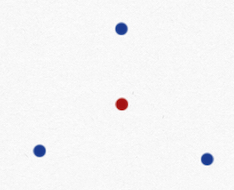
\includegraphics[width=20mm]{f1}
  \caption{4 points that can't be shattered by axis aligned rectangles}\label{f1}
  \end{figure}
  When the blue points are +1 and the red point is -1, this can't be realized by any axis aligned rectangle. But according to the definition, as long as we find 4 points that can be shattered by $\mcH$, $VCdim(\mcH)\geq 4$. We find:
  
  \begin{figure}[H]
  \centering
  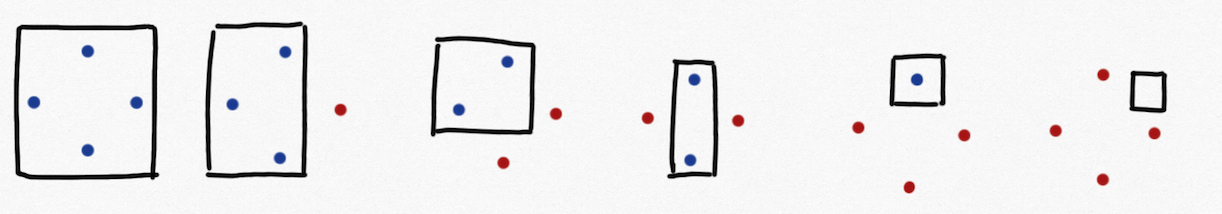
\includegraphics[width=120mm]{f2}
  \caption{4 points that can be shattered by axis aligned rectangles}\label{f2}
  \end{figure}
  In Figure \ref{f2}, blue points are given label +1 and red points are given label -1. Figure \ref{f2} shows how different combinations of labels can be realized by axis aligned rectangles. This shows that $VCdim \geq 4$. To show any 5 points can't be shattered, let's consider any 5 points $S={p_1, p_2, p_3, p_4, p_5}$. From $S$, take a leftmost point, a rightmost point, a lowest point, and a highest point. Without loss of generality, let $p_5$ be the point that was not selected(there might be several points that are not selected but we can just choose one). Now, define the labeling (1,1,1,1,0). It is impossible to obtain this labeling by an axis aligned rectangle. Indeed, such a rectangle must contain $p_1, p_2, p_3, p_4$, but in this case the rectangle must contain $p_5$ as well, because its coordinates are within the intervals defined by the selected points. So, $S$ is not shattered by $\mcH$, and therefore $VCdim(\mcH) = 4$.
\end{example}
To give a uniform convergence bound by VC dimension, we first build the relationship between VC dimension and growth function, then use Theorem \ref{t1}.
\begin{lemma}(Sauer-Shelah-VC Lemma)
	If $VCdim(\mcH)=D$, then:
	\begin{displaymath}
  		\Gamma_\mcH(m) \leq \sum_{i=0}^D\binom m i \leq (\frac{em}{D})^D
	\end{displaymath}
\end{lemma}
Figure \ref{f3} plots the growth function and $2^m$. When the sample size m is smaller than VC dimension, the growth function grows exponentially with m. After the sample size m reaches VC dimension, the growth function grows much more slowly(polynomially) with m.
\begin{figure}[H]
  \centering
  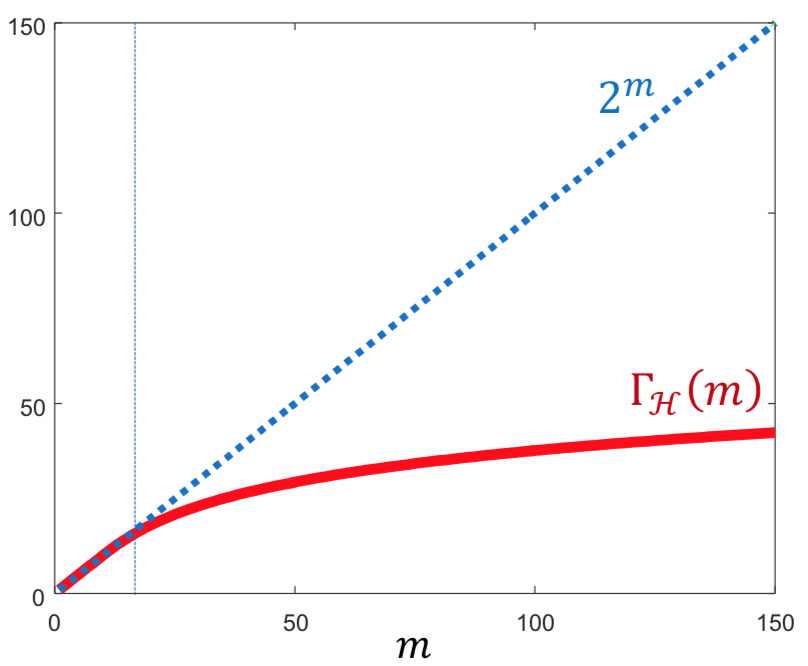
\includegraphics[width=70mm]{f3}
  \caption{Plotting growth function and $2^m$}\label{f3}
\end{figure}
From Sauer Lemma, we get:
\begin{displaymath}
  \log{|\Gamma_\mcH(2m)|} \leq \log{(\frac{em}{VCdim})^{VCdim}} \leq O(VCdim\cdot \log{m})
\end{displaymath}
Plugging this into Theorem \ref{t1}, we obtain:

\begin{theorem}
\begin{displaymath}
	\forall^\delta_{S\sim\mcD^m},\ L_\mcD(\hat{h}) \leq L_S(\hat{h}) + O\left(\sqrt{\frac{VCdim(\mcH)\log{m}+\log{1/\delta}}{m}}\right)
\end{displaymath}
With a very complex proof, this can be improved to:
\begin{displaymath}
	\forall^\delta_{S\sim\mcD^m},\ L_\mcD(\hat{h}) \leq L_S(\hat{h}) + O\left(\sqrt{\frac{VCdim(\mcH)+\log{1/\delta}}{m}}\right)
\end{displaymath}
\end{theorem}
We now show more examples of VC dimension:
\begin{example}\label{excircle}(Circles in $\reals^2$)
	\begin{displaymath}
		\mcH = \{h_{c,r}=[[\parallel x-c \parallel\leq r]]| c\in\reals^2, r\in \reals \}
	\end{displaymath}
  \begin{figure}[H]
  \centering
  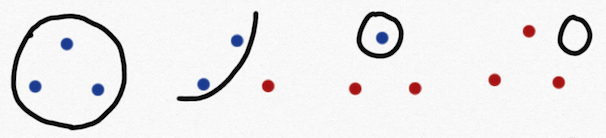
\includegraphics[width=80mm]{f4}
  \caption{3 points that can be shattered by circles}\label{f4}
  \end{figure}
	As shown in Figure \ref{f4}, where blue points are given +1 label and red points are given -1 label, circles can shatter 3 points. So $VCdim(\mcH)\geq 3$.
\end{example}

\begin{example}(Circles and their complement)
  \begin{figure}[H]
  \centering
  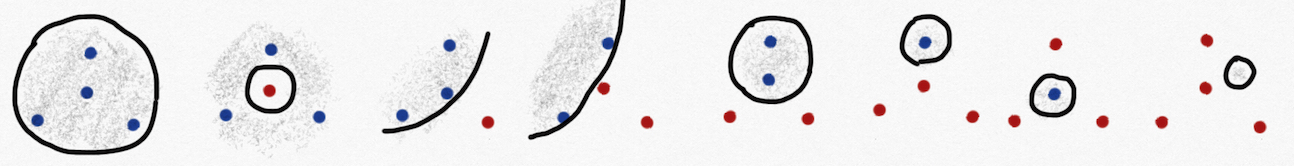
\includegraphics[width=130mm]{f5}
  \caption{3 points that can be shattered by circles and their complement}\label{f5}
  \end{figure}
	As shown in Figure \ref{f5}, where blue points are given +1 label, red points are given -1 label, and the regions of +1 label are in shadow, circles and their complement can shatter 4 points. So $VCdim(\mcH)\geq 4$.
\end{example}

\begin{example}(Circles around origin)
	\begin{displaymath}
		\mcH = \{h_r=[[\parallel x \parallel\leq r]]|r\in \reals \}
	\end{displaymath}
  \begin{figure}[H]
  \centering
  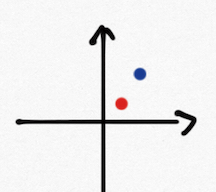
\includegraphics[width=30mm]{f6}
  \caption{2 points that can't be shattered by circles around origin}\label{f6}
  \end{figure}
	Apparently $\mcH$ can shatter 1 point. As shown in Figure \ref{f5}, any 2 points can't be shattered by circles around origin, because $\mcH$ can't produce the labeling where the point closer to the origin is -1 while the other is +1. So $VCdim(\mcH) = 1$.
\end{example}

\begin{example}(Axis aligned ellipses)
	\begin{displaymath}
		\mcH = \{h_{c,r}=[[\frac{(x[1]-c[1])^2}{r[1]^2}+\frac{(x[2]-c[2])^2}{r[2]^2}\leq 1]]| c, r\in\reals^2\}
	\end{displaymath}
  Can shatter 4 points, so $VCdim(\mcH)\geq 4$.
\end{example}

\begin{example}(General ellipses)
  Can shatter 5 points, so $VCdim(\mcH)\geq 5$.
\end{example}
\begin{example}(Homogeneous half spaces)
	\begin{displaymath}
  		\mcH_\phi = \{[[\langle w,\phi(x)\geq 0]]|w\in \reals^d\}, \qquad \phi:\mcX\rightarrow \reals^d
	\end{displaymath}
	$\mcH_\phi$ can shatter the d standard basis $e_1,...,e_d$ by choosing $w=(y_1, y_2,...,y_d)$.
	
	Now we prove the claim that $\mcH_\phi$ can't shatter any set of $d+1$ points.
	\begin{proof}
		For any $d+1$ points $x_1,...,x_{d+1}$, there must be some linear dependency:$\sum_ia_ix_i=0$. Consider the labeling $y_i=sign(a_i)$(arbitrary for $a_i=0$). If we can shatter, there's a predictor $w$ s.t.
		\begin{displaymath}
  			sign(\langle w, x_i\rangle)=y_i=sign(a_i)
		\end{displaymath}
		This implies that when $a_i \neq 0$,
		\begin{displaymath}
  			a_i\langle w, x_i\rangle >0
		\end{displaymath}
		We then have:
		\begin{displaymath}
  			\langle w, \sum_ia_ix_i\rangle = \sum_i a_i\langle w, x_i\rangle >0
		\end{displaymath}
		Which contradicts with the linear dependency:
		\begin{displaymath}
  			\langle w, \sum_ia_ix_i\rangle = 0
		\end{displaymath}
	\end{proof}
	Since $\mcH_\phi$ can shatter $d$ points but not $d+1$ points, $VCdim(\mcH_\phi)=d$
\end{example}
Based on the above result, we have the following half space representation theorem:
\begin{theorem}\label{t3}(half space representation)
	For a hypothesis class $\mcH$, if there exists $\phi:\mcX \rightarrow \reals^D$ s.t.
	\begin{displaymath}
  		\mcH \subseteq \mcH_\phi,
	\end{displaymath}
	i.e. every hypothesis $h\in \mcH$ can be written as $h(x)=sign(\langle w, \phi(x)\rangle)$ for some $w_h \in \reals^D$, then $VCdim(\mcH)\leq D$.
\end{theorem}
\begin{example}
	Non-homogeneous half-spaces over $\reals^d$ can be represented by $(d+1)$-dimension homogeneous half-spaces with $\tilde{\phi}(x)=[\phi(x),1]$
\end{example}
\begin{example}
	A circle can be represented by a 4-dimension half-space:
	\begin{displaymath}
	\begin{aligned}
  		h_{a,r}(x){} & =[[(x[1]-a[1])^2+(x[2]-a[2])^2\leq r^2]] \\
  		& =[[x[1]^2-2a[1]x[1]+a[1]^2+x[2]^2-2a[2]x[2]+a[2]^2\leq r^2]] \\
  		& =sign((-x[1]^2-x[2]^2)+2a[1]x[1]+2a[2]x[2]+(r^2-a[1]^2-a[2]^2)1) \\
  		& =sign(\langle w_{a,r}, \phi(x)\rangle)
  	\end{aligned}
	\end{displaymath}
	where $\phi(x)=(-x[1]^2-x[2]^2, x[1], x[2], 1)$ and $w_{a,r}=(1,2a[1], 2a[2], r^2-a[1]^2-a[2]^2)$. According to Theorem \ref{t3}, $VCdim\leq 4$. We showed in Example \ref{excircle} that the lower bound of VC dimension is 3, so why isn't the upper bound tight? Notice that $w[1]$ is restricted to 1. In fact, if we allow $w[1]<0$, we get circles and their complement(including half-spaces, which can be thought of as infinite radius circles), and half space representation gives a tight bound on VC dimension($VCdim=4$).
\end{example}

\begin{example}(Axis-aligned ellipses and their complement)
	\begin{displaymath}
  		\phi(x)=(x[1]^2, x[2]^2, x[1], x[2], 1)
	\end{displaymath}
	$VCdim\leq 5$
\end{example}

\begin{example}(Conic cuts (including all ellipses))
	\begin{displaymath}
  		\phi(x)=(x[1]^2, x[2]^2, x[1]x[2], x[1], x[2], 1)
	\end{displaymath}
	$VCdim\leq 6$
\end{example}

\begin{example}(Degree-k polynomials over $\reals^2$)
	\begin{displaymath}
	\begin{aligned}
  		\phi(x)={} & (x[1]^k, x[1]^{k-1}x[2]^1, ..., x[1]^1x[2]^{k-1}, x[2]^k, \\
  		& x[1]^{k-1}, x[1]^{k-2}x[2]^1, ..., x[1]^1x[2]^{k-2}, x[2]^{k-1}, \\
  		& x[1]^{k-2},... \\
  		& x[1]^{2}, x[1]x[2], x[2]^{2}, \\
  		& x[1], x[2], 1) \in \reals^{(k+1)(k+2)/2}
  	\end{aligned}
	\end{displaymath}
	$VCdim\leq (k+1)(k+2)/2$
\end{example}
\begin{example}(Degree-k polynomials over $\reals^d$)
	\begin{displaymath}
		\phi(x) \in \reals^{\binom {d+k-1} k}
	\end{displaymath}
	$VCdim\leq O(d^k)$
\end{example}
In the previous examples, the VC dimension happened to equal the number of parameters defining the hypothesis class, which makes us to think about this question: is VC dimension always equal to the number of parameters? The answer is yes when we are dealing with most "normal" hypothesis classes. But it isn't always the case. Look at the following counter example:
\begin{example}
	\begin{displaymath}
		\mcX = \reals \qquad \mcH=\{h_{\theta,v}(x)=sign(sin(vx+\theta))|v,\theta\in \reals\}
	\end{displaymath}
	We now prove that $VCdim(\mcH)=\infty$:
	\begin{proof}
		Consider the infinite set of points $\{x_i=10^{-i}\}_{i=1,2,...}$. Any labeling $y_1,y_2,...$ can be obtained by $\theta=0$ and:
		\begin{displaymath}
  			v=\pi\left(1-\sum^\infty_{i=1}\frac{y_i}{2x_i}\right)
		\end{displaymath}
	\end{proof}
\end{example}
Back to learning, we have shown that the sample complexity of ERM can be given by cardinality and VC dimension:
\begin{displaymath}
  m_{ERM,\mcH}(\epsilon, \delta)=O\left(\frac{\log{|\mcH|}+\log{1/\delta}}{\epsilon^2}\right)
\end{displaymath}
\begin{displaymath}
  m_{ERM,\mcH}(\epsilon, \delta)=O\left(\frac{VCdim(\mcH)+\log{1/\delta}}{\epsilon^2}\right)
\end{displaymath}
We can still ask these questions: Can a class with infinite VC-dimension be learnable? Can the sample complexity be lower than the VC dimension? We have shown what is learnable, but we haven't shown what is not learnable. Are there any hypothesis classes that are not learnable? Can we learn the class $\mcH=\mcY^\mcX$ of all possible predictors?
\subsection{Statistical No Free Lunch}
In this section will prove that there's no learning rule that can succeed on all source distributions.
\begin{theorem}(Statistical No Free Lunch)
	For any domain $\mcX$ of size $|\mcX|$ and any learning rule $A$, there exists a source distribution $\mcD$ with $\mathbb{P}_{x,y\sim\mcD}[f(x)=y]=1$ for some $f:\mcX\rightarrow\{\pm1\}$, such that for $m<\frac{|X|}{2}$,
	 \begin{displaymath}
  		\mathbb{E}_{S\sim\mcD^m}[L_\mcD(A(S))]\geq \frac{1}{4}
	\end{displaymath}
	and so $w.p.\geq1/7,\ L_\mcD(A(S))\geq1/8$.
	
	For an infinite domain $\mcX$, for any learning rule $A$ and any sample size $m$, there exists a source distribution and $f$ as above such that
	\begin{displaymath}
  		\mathbb{E}_{S\sim\mcD^m}[L_\mcD(A(S))]\geq \frac{1}{4}
	\end{displaymath}
\end{theorem}
Instead of proving Statistical No Free Lunch Theorem, we prove a stronger statement:
\begin{theorem}
	For a finite domain $\mcX,\ \mcY=\{\pm1\}$, any learning rule $A$ and any sample size $m$, 
	\begin{displaymath}
  		\frac{1}{2}-\frac{m}{2|\mcX|}\leq \mathbb{E}_f\mathbb{E}_{S\sim \mcU^m_f}[L_{\mcU_f}(A(S))]\leq \frac{1}{2}+\frac{m}{2|\mcX|}
	\end{displaymath}
	The first expectation is taken over a uniform distribution of $f:\mcX\rightarrow\mcY$ where for each $x$ set, w.p. $1/2 ,\ f(x)=\pm1$, independent of all other values. The second expectation is taken over samples of size $m$ from $\mcU_f$, which is the source distribution s.t. $x$ is uniform over $\mcX$ and $y=f(x)$ with probability one.
\end{theorem}
Before proving this theorem, we define:
\begin{defn}
	$S$ is consistent with $f$ if $\forall_{(x_i,y_i)\in S}f(x_i)=y_i$. S is self-consistent if it is consistent with some $f$ (i.e. if $x_i=x_j$ then $y_i=y_j$).
\end{defn}
\begin{proof}
	For any learning rule $A$, and any self-consistent sample $S$:
	\begin{displaymath}
  	\begin{aligned}
  		{} & \mathbb{E}_f[L_{\mcU_f}(A(S))| S\ cons\ with\ f] \\
  		& =\mathbb{E}_f[\frac{1}{|\mcX|}\sum_x[[A(S)(x)\neq f(x)]]| S\ cons\ with\ f] \\
  		& = \frac{1}{|\mcX|}\left(\sum_{x\in S}\mathbb{P}_f[A(S)(x)\neq f(x)]+\sum_{x\notin S}\mathbb{P}_f[A(S)(x)\neq f(x)]\right)
  	\end{aligned}
	\end{displaymath}
	For $x$ that appears in sample $S$, the best a learning rule can do is to get all of these $x$ right, and the worst case is when a learning rule gets all of these $x$ wrong. For $x$ that doesn't appear in sample $S$, learning rules have no information of it, so by taking expectation over all consistent f, all learning rule can get half of these $x$ right (since f divides the labels into $\pm1$ with equal probability). So $\frac{1}{2}-\frac{m'}{2|\mcX|}\leq \mathbb{E}_f[L_{\mcU_f}(A(S))| S\ cons\ with\ f] \leq \frac{1}{2}+\frac{m'}{2|\mcX|}$, where $m'=|\{x|x\in S\}|$. And so:
	\begin{displaymath}
  	\begin{aligned}
  		\mathbb{E}_f\mathbb{E}_{S\sim \mcU^m_f}[L_{\mcU_f}(A(S))] {} & =\mathbb{E}_f\mathbb{E}_{self-cons\ S}[L_{\mcU_f}(A(S))| S\ cons\ with\ f] \\
  		& =\mathbb{E}_{self-cons\ S}\mathbb{E}_f[L_{\mcU_f}(A(S))| S\ cons\ with\ f] \\
  	\end{aligned}
	\end{displaymath}
	\begin{displaymath}
  		\frac{1}{2}-\frac{m}{2|\mcX|}\leq \mathbb{E}_f\mathbb{E}_{S\sim \mcU^m_f}[L_{\mcU_f}(A(S))]\leq \frac{1}{2}+\frac{m}{2|\mcX|}
	\end{displaymath}
\end{proof}
Finally, we can use Statistical No Free Lunch Theorem to show that the class $\mcH=\mcY^\mcX$ is not learnable for infinite $\mcX$; For finite $\mcX$, sample complexity is $m_{\mcY^\mcX}(1/8, 6/7)\geq \Omega(|\mcX|)=\Omega(VCdim(\mcH))=\Omega(\log{|\mcH|})$
\end{document}